% In-Context Gibbs — journal version for IEEE Transactions on Pattern Analysis and Machine Intelligence (TPAMI).
% IEEE Computer Society template: IEEEtran.cls V1.8b, options [10pt,journal,compsoc] (style_ieee/SOURCE.txt).
% All appendices are supplemental material in a separate PDF (supplement.tex), as the IEEE CS author guidelines require;
% cross-references between the two files use xr-hyper. Build: make  (runs both files in the right order).
% Every number in the text comes from numbers*.tex / tables/*.tex, generated by the scripts in scripts/ from the
% registered analysis outputs. Do not type numbers by hand. The TMLR version is commit 0b425e2.
\documentclass[10pt,journal,compsoc]{IEEEtran}
\usepackage[numbers,sort&compress]{natbib}
\usepackage[utf8]{inputenc}
\usepackage{amsmath,amssymb,amsthm}
\usepackage{booktabs,multirow,threeparttable,array}
\usepackage{graphicx}
\usepackage{placeins}
\usepackage[dvipsnames]{xcolor}
\usepackage{microtype}
\usepackage{nicefrac}
\usepackage{algorithm}
\usepackage[noend]{algpseudocode}
\usepackage{xr-hyper}
\usepackage[colorlinks=true,linkcolor=MidnightBlue,citecolor=MidnightBlue,urlcolor=MidnightBlue]{hyperref}
\usepackage[capitalise,noabbrev]{cleveref}
\externaldocument[][nocite]{supplement}[]
\crefname{appendix}{Appendix}{Appendices}

\setlength{\emergencystretch}{1.5em}
\setcounter{secnumdepth}{3}  % IEEEtran numbers \paragraph otherwise
% generated by paper/scripts/make_tables.py — do not edit
\makeatletter
\@namedef{v@s1-h3-cells}{128}
\@namedef{v@s1-h3-frac}{86.7\%}
\@namedef{v@s1-h3-rho}{0.36}
\@namedef{v@s1-llp-cmp-ci}{[\ensuremath{-}0.013, +0.057]}
\@namedef{v@s1-llp-cmp-diff}{+0.024}
\@namedef{v@s1-llp-cmp-n}{10}
\@namedef{v@s1-llp-cmp-p}{0.232}
\@namedef{v@s1-llp-cmp-prel}{\ensuremath{=}0.232}
\@namedef{v@s1-llp-cmp-w}{8}
\@namedef{v@s1-llp-cmp-wtl}{8/0/2}
\@namedef{v@s1-llp-mean-dllplin_def}{0.831}
\@namedef{v@s1-llp-mean-gibbs_warm}{0.855}
\@namedef{v@s1-llp-mean-hard_em_warm}{0.854}
\@namedef{v@s1-llp-mean-naive}{0.707}
\@namedef{v@s1-llp-mean-oracle}{0.923}
\@namedef{v@s1-llp-naive-ci}{[+0.099, +0.201]}
\@namedef{v@s1-llp-naive-diff}{+0.148}
\@namedef{v@s1-llp-naive-n}{10}
\@namedef{v@s1-llp-naive-p}{0.004}
\@namedef{v@s1-llp-naive-prel}{\ensuremath{=}0.004}
\@namedef{v@s1-llp-naive-w}{10}
\@namedef{v@s1-llp-naive-wtl}{10/0/0}
\@namedef{v@s1-n-binary}{10}
\@namedef{v@s1-n-multi}{14}
\@namedef{v@s1-pll3-cmp-ci}{[+0.005, +0.044]}
\@namedef{v@s1-pll3-cmp-diff}{+0.022}
\@namedef{v@s1-pll3-cmp-n}{14}
\@namedef{v@s1-pll3-cmp-p}{0.084}
\@namedef{v@s1-pll3-cmp-prel}{\ensuremath{=}0.084}
\@namedef{v@s1-pll3-cmp-w}{10}
\@namedef{v@s1-pll3-cmp-wtl}{10/0/4}
\@namedef{v@s1-pll3-mean-cc_tun}{0.824}
\@namedef{v@s1-pll3-mean-gibbs_warm}{0.847}
\@namedef{v@s1-pll3-mean-hard_em_warm}{0.847}
\@namedef{v@s1-pll3-mean-naive}{0.748}
\@namedef{v@s1-pll3-mean-oracle}{0.863}
\@namedef{v@s1-pll3-naive-ci}{[+0.049, +0.163]}
\@namedef{v@s1-pll3-naive-diff}{+0.099}
\@namedef{v@s1-pll3-naive-n}{14}
\@namedef{v@s1-pll3-naive-p}{\ensuremath{<}0.001}
\@namedef{v@s1-pll3-naive-prel}{\ensuremath{<}0.001}
\@namedef{v@s1-pll3-naive-w}{13}
\@namedef{v@s1-pll3-naive-wtl}{13/0/1}
\@namedef{v@s1-pll6-cmp-ci}{[\ensuremath{-}0.301, +0.002]}
\@namedef{v@s1-pll6-cmp-diff}{\ensuremath{-}0.132}
\@namedef{v@s1-pll6-cmp-n}{14}
\@namedef{v@s1-pll6-cmp-p}{0.715}
\@namedef{v@s1-pll6-cmp-prel}{\ensuremath{=}0.715}
\@namedef{v@s1-pll6-cmp-w}{7}
\@namedef{v@s1-pll6-cmp-wtl}{7/0/7}
\@namedef{v@s1-pll6-mean-cc_tun}{0.793}
\@namedef{v@s1-pll6-mean-gibbs_warm}{0.661}
\@namedef{v@s1-pll6-mean-hard_em_warm}{0.573}
\@namedef{v@s1-pll6-mean-naive}{0.481}
\@namedef{v@s1-pll6-mean-oracle}{0.863}
\@namedef{v@s1-pll6-naive-ci}{[+0.106, +0.261]}
\@namedef{v@s1-pll6-naive-diff}{+0.180}
\@namedef{v@s1-pll6-naive-n}{14}
\@namedef{v@s1-pll6-naive-p}{0.002}
\@namedef{v@s1-pll6-naive-prel}{\ensuremath{=}0.002}
\@namedef{v@s1-pll6-naive-w}{12}
\@namedef{v@s1-pll6-naive-wtl}{12/0/2}
\@namedef{v@s2-h3-cells}{38}
\@namedef{v@s2-h3-frac}{78.9\%}
\@namedef{v@s2-h3-prope}{0.00}
\@namedef{v@s2-h3-rho}{0.66}
\@namedef{v@s2-llp-cmp-ci}{[+0.024, +0.086]}
\@namedef{v@s2-llp-cmp-diff}{+0.052}
\@namedef{v@s2-llp-cmp-n}{18}
\@namedef{v@s2-llp-cmp-p}{\ensuremath{<}0.001}
\@namedef{v@s2-llp-cmp-prel}{\ensuremath{<}0.001}
\@namedef{v@s2-llp-cmp-w}{16}
\@namedef{v@s2-llp-cmp-wtl}{16/0/2}
\@namedef{v@s2-llp-mean-dllp_tun}{0.799}
\@namedef{v@s2-llp-mean-dllplin_def}{0.788}
\@namedef{v@s2-llp-mean-gibbs_warm}{0.840}
\@namedef{v@s2-llp-mean-hard_em_warm}{0.827}
\@namedef{v@s2-llp-mean-naive}{0.724}
\@namedef{v@s2-llp-mean-oracle}{0.879}
\@namedef{v@s2-llp-naive-ci}{[+0.085, +0.150]}
\@namedef{v@s2-llp-naive-diff}{+0.116}
\@namedef{v@s2-llp-naive-n}{18}
\@namedef{v@s2-llp-naive-p}{\ensuremath{<}0.001}
\@namedef{v@s2-llp-naive-prel}{\ensuremath{<}0.001}
\@namedef{v@s2-llp-naive-w}{18}
\@namedef{v@s2-llp-naive-wtl}{18/0/0}
\@namedef{v@s2-llp-oracle-gap}{0.039}
\@namedef{v@s2-llp-strongest-frac}{89\%}
\@namedef{v@s2-llp-strongest-name}{tuned DLLP (MLP)}
\@namedef{v@s2-llp-strongest-wins}{16/18}
\@namedef{v@s2-n-binary}{18}
\@namedef{v@s2-n-multi}{10}
\@namedef{v@s2-n-total}{28}
\@namedef{v@s2-pll3-cmp-ci}{[+0.006, +0.019]}
\@namedef{v@s2-pll3-cmp-diff}{+0.012}
\@namedef{v@s2-pll3-cmp-n}{10}
\@namedef{v@s2-pll3-cmp-p}{0.016}
\@namedef{v@s2-pll3-cmp-prel}{\ensuremath{=}0.016}
\@namedef{v@s2-pll3-cmp-w}{8}
\@namedef{v@s2-pll3-cmp-wtl}{8/2/0}
\@namedef{v@s2-pll3-mean-cc_tun}{0.850}
\@namedef{v@s2-pll3-mean-gibbs_warm}{0.862}
\@namedef{v@s2-pll3-mean-hard_em_warm}{0.862}
\@namedef{v@s2-pll3-mean-naive}{0.840}
\@namedef{v@s2-pll3-mean-oracle}{0.870}
\@namedef{v@s2-pll3-naive-ci}{[+0.012, +0.033]}
\@namedef{v@s2-pll3-naive-diff}{+0.022}
\@namedef{v@s2-pll3-naive-n}{10}
\@namedef{v@s2-pll3-naive-p}{0.008}
\@namedef{v@s2-pll3-naive-prel}{\ensuremath{=}0.008}
\@namedef{v@s2-pll3-naive-w}{10}
\@namedef{v@s2-pll3-naive-wtl}{10/0/0}
\@namedef{v@s2-pll3-oracle-gap}{0.8}
\@namedef{v@s2-pll3-rule60}{10/10}
\@namedef{v@s2-pll6-cmp-ci}{[+0.006, +0.019]}
\@namedef{v@s2-pll6-cmp-diff}{+0.012}
\@namedef{v@s2-pll6-cmp-n}{10}
\@namedef{v@s2-pll6-cmp-p}{0.016}
\@namedef{v@s2-pll6-cmp-prel}{\ensuremath{=}0.016}
\@namedef{v@s2-pll6-cmp-w}{8}
\@namedef{v@s2-pll6-cmp-wtl}{8/1/1}
\@namedef{v@s2-pll6-mean-cc_tun}{0.839}
\@namedef{v@s2-pll6-mean-gibbs_warm}{0.851}
\@namedef{v@s2-pll6-mean-hard_em_warm}{0.803}
\@namedef{v@s2-pll6-mean-naive}{0.647}
\@namedef{v@s2-pll6-mean-oracle}{0.870}
\@namedef{v@s2-pll6-mean-rc_tun}{0.839}
\@namedef{v@s2-pll6-naive-ci}{[+0.094, +0.337]}
\@namedef{v@s2-pll6-naive-diff}{+0.205}
\@namedef{v@s2-pll6-naive-n}{10}
\@namedef{v@s2-pll6-naive-p}{0.008}
\@namedef{v@s2-pll6-naive-prel}{\ensuremath{=}0.008}
\@namedef{v@s2-pll6-naive-w}{10}
\@namedef{v@s2-pll6-naive-wtl}{10/0/0}
\@namedef{v@s2-pll6-oracle-gap}{1.9}
\@namedef{v@s2-pll6-rule60}{9/10}
\newcommand{\val}[1]{\@ifundefined{v@#1}{\textbf{\textcolor{red}{??#1}}}{\@nameuse{v@#1}}}
\makeatother

% generated by paper/scripts/make_appendix.py — do not edit
\makeatletter
\@namedef{v@rq1-e1-n}{14}
\@namedef{v@rq1-e1-tvmax}{3\times10^{-14}}
\@namedef{v@rq1-e3-n}{30}
\@namedef{v@rq1-e5-nmax}{1{,}000}
\@namedef{v@rq1-e5-pred-all-n1000}{1.7\times10^{-4}}
\@namedef{v@rq1-e5-pred-free-n1000}{0.031}
\@namedef{v@rq1-loose-max}{15}
\@namedef{v@rq1-loose-median}{3.9}
\@namedef{v@rq1-loose-min}{1.9}
\@namedef{v@rq1-pfn-final-single}{0.012}
\@namedef{v@rq1-pfn-final-swap}{0.007}
\@namedef{v@rq1-thm2-held}{42}
\@namedef{v@rq1-thm2-n}{42}
\@namedef{v@s1-d1-p}{0.039}
\@namedef{v@s1-d2-p}{0.010}
\@namedef{v@s1-d3-max}{\ensuremath{-}0.013}
\@namedef{v@s1-noise2-naive-diff}{\ensuremath{-}0.013}
\@namedef{v@s1-noise2-naive-wtl}{1/0/9}
\@namedef{v@s1-noise4-naive-diff}{\ensuremath{-}0.054}
\@namedef{v@s1-noise4-naive-wtl}{1/0/9}
\@namedef{v@s1-nolose-nlev}{6}
\@namedef{v@s1-nolose-nneg}{6}
\@namedef{v@s1-puscar1-naive-diff}{\ensuremath{-}0.033}
\@namedef{v@s1-puscar1-naive-wtl}{5/0/5}
\@namedef{v@s1-puscar3-naive-diff}{\ensuremath{-}0.028}
\@namedef{v@s1-puscar3-naive-wtl}{2/0/8}
\@namedef{v@s1-ssl20-naive-diff}{\ensuremath{-}0.016}
\@namedef{v@s1-ssl20-naive-wtl}{0/0/10}
\@namedef{v@s1-ssl5-naive-diff}{\ensuremath{-}0.041}
\@namedef{v@s1-ssl5-naive-wtl}{0/0/10}
\@namedef{v@s1-tabicl-oracle-maxdiff}{0.005}
\makeatother

% generated by paper/scripts/make_v2.py — do not edit
\makeatletter
\@namedef{v@all-n-datasets}{72}
\@namedef{v@s1-fin-icl-min}{0.925}
\@namedef{v@s1-fin-pfn-mfeat}{0.16--0.17}
\@namedef{v@s1-fin-pfn-mice}{0.44--0.64}
\@namedef{v@s1-fin-pfn-mice-max}{0.64}
\@namedef{v@s1-fin-pfn-opt}{0.27, 0.89, 0.93}
\@namedef{v@s1-fin-pfn-opt-high}{2}
\@namedef{v@s1-fin-pfn-semeion}{0.34--0.37}
\@namedef{v@s1-rising-list}{TabPFN~v2, semeion: 3 of 3; TabPFN~v2, MiceProtein: 3 of 3; TabPFN~v2, optdigits: 2 of 3; TabICL~v2, MiceProtein: 2 of 3}
\@namedef{v@s1-start-tabiclv2-MiceProtein}{0.31}
\@namedef{v@s1-start-tabiclv2-mfeat-factors}{0.26}
\@namedef{v@s1-start-tabiclv2-optdigits}{0.31}
\@namedef{v@s1-start-tabiclv2-semeion}{0.32}
\@namedef{v@s1-start-tabpfnv2-MiceProtein}{0.22}
\@namedef{v@s1-start-tabpfnv2-mfeat-factors}{0.16}
\@namedef{v@s1-start-tabpfnv2-optdigits}{0.17}
\@namedef{v@s1-start-tabpfnv2-semeion}{0.17}
\@namedef{v@s2-llp-strongest-ci}{[+0.018, +0.072]}
\@namedef{v@s2-llp-strongest-diff}{+0.041}
\@namedef{v@s2-mean-gibbs-llp}{0.840}
\@namedef{v@s2-mean-gibbs-pll3}{0.862}
\@namedef{v@s2-mean-gibbs-pll6}{0.851}
\@namedef{v@s2-mean-hardem-llp}{0.827}
\@namedef{v@s2-mean-hardem-pll3}{0.862}
\@namedef{v@s2-mean-hardem-pll6}{0.803}
\@namedef{v@s2-mean-sem-llp}{0.835}
\@namedef{v@s2-mean-sem-pll3}{0.858}
\@namedef{v@s2-mean-sem-pll6}{0.843}
\@namedef{v@s2-pll3-cmp-ci4}{[+0.0065, +0.0192]}
\@namedef{v@s2-pll3-cmp-diff4}{+0.0125}
\@namedef{v@s2-pll6-cmp-ci4}{[+0.0056, +0.0193]}
\@namedef{v@s2-pll6-cmp-diff4}{+0.0121}
\@namedef{v@s3-A1-tabdpt-llp}{0.799}
\@namedef{v@s3-A1-tabdpt-pll}{0.720}
\@namedef{v@s3-A1-tabicl_v2-llp}{0.803}
\@namedef{v@s3-A1-tabicl_v2-pll}{0.805}
\@namedef{v@s3-A1-tabpfn_v2-llp}{0.798}
\@namedef{v@s3-A1-tabpfn_v2-pll}{0.494}
\@namedef{v@s3-A1-tabpfn_v3-llp}{0.817}
\@namedef{v@s3-A1-tabpfn_v3-pll}{0.650}
\@namedef{v@s3-G-tabdpt}{+0.037}
\@namedef{v@s3-G-tabicl_v2}{+0.024}
\@namedef{v@s3-G-tabpfn_v2}{+0.013}
\@namedef{v@s3-G-tabpfn_v3}{+0.112}
\@namedef{v@s3-L-llp}{0.783}
\@namedef{v@s3-L-pll}{0.717}
\@namedef{v@s3-R-tabdpt}{3}
\@namedef{v@s3-R-tabicl_v2}{1}
\@namedef{v@s3-R-tabpfn_v2}{2}
\@namedef{v@s3-R-tabpfn_v3}{4}
\@namedef{v@s3-X-llp}{0.828}
\@namedef{v@s3-X-pll}{0.808}
\@namedef{v@s3-a1L-mean}{+0.018}
\@namedef{v@s3-a1L-p}{0.14}
\@namedef{v@s3-a1L-wl}{14/6}
\@namedef{v@s3-c4-both}{1}
\@namedef{v@s3-c4-n}{10}
\@namedef{v@s3-c4-rate}{14.1\%}
\@namedef{v@s3-c4-v1-reg}{14}
\@namedef{v@s3-c4-vs-L}{9}
\@namedef{v@s3-c4-vs-L-rate}{12.7\%}
\@namedef{v@s3-c4-vs-v1}{2}
\@namedef{v@s3-c5-gap}{0.000}
\@namedef{v@s3-c5-nlose}{1}
\@namedef{v@s3-c5-worst-X}{0.645}
\@namedef{v@s3-c5-worst-best}{0.671}
\@namedef{v@s3-c5-worst-name}{micro-mass}
\@namedef{v@s3-excl-ids}{176}
\@namedef{v@s3-flag-n}{5}
\@namedef{v@s3-flip-cells}{4}
\@namedef{v@s3-flip-range}{0.30--0.49}
\@namedef{v@s3-h1-ci}{[+0.016, +0.114]}
\@namedef{v@s3-h1-l}{1}
\@namedef{v@s3-h1-llp}{+0.007}
\@namedef{v@s3-h1-mean}{+0.058}
\@namedef{v@s3-h1-median}{+0.003}
\@namedef{v@s3-h1-p}{\ensuremath{<}0.001}
\@namedef{v@s3-h1-pll}{+0.136}
\@namedef{v@s3-h1-prel}{\ensuremath{<}0.001}
\@namedef{v@s3-h1-w}{13}
\@namedef{v@s3-h1-wtl}{13/6/1}
\@namedef{v@s3-h2-ci}{[+0.019, +0.079]}
\@namedef{v@s3-h2-l}{0}
\@namedef{v@s3-h2-llp}{+0.021}
\@namedef{v@s3-h2-mean}{+0.046}
\@namedef{v@s3-h2-median}{+0.016}
\@namedef{v@s3-h2-p}{\ensuremath{<}0.001}
\@namedef{v@s3-h2-pll}{+0.083}
\@namedef{v@s3-h2-prel}{\ensuremath{<}0.001}
\@namedef{v@s3-h2-top}{micro-mass (+0.24), cnae-9 (+0.20), vowel (+0.17)}
\@namedef{v@s3-h2-w}{18}
\@namedef{v@s3-h2-wtl}{18/2/0}
\@namedef{v@s3-h3-auc}{0.766}
\@namedef{v@s3-h3-auc-tabdpt}{0.59}
\@namedef{v@s3-h3-auc-tabicl_v2}{0.85}
\@namedef{v@s3-h3-auc-tabpfn_v2}{0.64}
\@namedef{v@s3-h3-auc-tabpfn_v3}{0.93}
\@namedef{v@s3-h3-ci}{[0.59, 0.92]}
\@namedef{v@s3-h3-nneg}{147}
\@namedef{v@s3-h3-npos}{66}
\@namedef{v@s3-meanA1-llp}{0.807}
\@namedef{v@s3-meanA1-pll}{0.725}
\@namedef{v@s3-meanv1-llp}{0.801}
\@namedef{v@s3-meanv1-pll}{0.589}
\@namedef{v@s3-n-binary}{12}
\@namedef{v@s3-n-cells}{213}
\@namedef{v@s3-n-multi}{8}
\@namedef{v@s3-n-pairs}{71}
\@namedef{v@s3-n-pfn2}{11}
\@namedef{v@s3-n-total}{20}
\@namedef{v@s3-pfn2-nllp}{10}
\@namedef{v@s3-pfn2-npll}{1}
\@namedef{v@s3-reg-Lbetter-n}{9}
\@namedef{v@s3-reg-v1stall-n}{8}
\@namedef{v@s3-review-dup}{1}
\@namedef{v@s3-review-keep}{20}
\@namedef{v@s3-review-n}{43}
\@namedef{v@s3-review-source}{14}
\@namedef{v@s3-review-syn}{8}
\@namedef{v@s3-s1-h1-mean}{+0.062}
\@namedef{v@s3-s1-h1-p}{0.003}
\@namedef{v@s3-s1-h1-wtl}{10/4/1}
\@namedef{v@s3-s1-h2-mean}{+0.044}
\@namedef{v@s3-s1-h2-p}{\ensuremath{<}0.001}
\@namedef{v@s3-s1-h2-wtl}{13/2/0}
\@namedef{v@s3-s1-n}{15}
\@namedef{v@s3-sub-n}{6}
\@namedef{v@s3-tabdpt-ids}{123}
\@namedef{v@s3-v1-tabdpt-llp}{0.786}
\@namedef{v@s3-v1-tabdpt-pll}{0.648}
\@namedef{v@s3-v1-tabicl_v2-llp}{0.802}
\@namedef{v@s3-v1-tabicl_v2-pll}{0.749}
\@namedef{v@s3-v1-tabpfn_v2-llp}{0.784}
\@namedef{v@s3-v1-tabpfn_v2-pll}{0.488}
\@namedef{v@s3-v1-tabpfn_v3-llp}{0.817}
\@namedef{v@s3-v1-tabpfn_v3-pll}{0.371}
\@namedef{v@s3x-A1-L-tabdpt}{+0.011}
\@namedef{v@s3x-A1-L-tabdpt-wtl}{14/0/6}
\@namedef{v@s3x-A1-L-tabicl_v2}{+0.047}
\@namedef{v@s3x-A1-L-tabicl_v2-wtl}{18/0/2}
\@namedef{v@s3x-A1-L-tabpfn_v2}{+0.023}
\@namedef{v@s3x-A1-L-tabpfn_v2-wtl}{8/0/3}
\@namedef{v@s3x-A1-L-tabpfn_v3}{\ensuremath{-}0.006}
\@namedef{v@s3x-A1-L-tabpfn_v3-wtl}{15/0/5}
\@namedef{v@s3x-A1L-A1}{+0.021}
\@namedef{v@s3x-A1L-A1-p}{0.005}
\@namedef{v@s3x-A1L-A1-wtl}{14/2/4}
\@namedef{v@s3x-X-A1-tabdpt}{+0.053}
\@namedef{v@s3x-X-A1-tabdpt-p}{\ensuremath{<}0.001}
\@namedef{v@s3x-X-A1-tabdpt-wtl}{16/2/2}
\@namedef{v@s3x-X-A1-tabicl_v2}{+0.016}
\@namedef{v@s3x-X-A1-tabicl_v2-p}{0.08}
\@namedef{v@s3x-X-A1-tabicl_v2-wtl}{10/5/5}
\@namedef{v@s3x-X-A1-tabpfn_v2}{+0.017}
\@namedef{v@s3x-X-A1-tabpfn_v2-p}{0.05}
\@namedef{v@s3x-X-A1-tabpfn_v2-wtl}{8/1/2}
\@namedef{v@s3x-X-A1-tabpfn_v3}{+0.070}
\@namedef{v@s3x-X-A1-tabpfn_v3-p}{0.004}
\@namedef{v@s3x-X-A1-tabpfn_v3-wtl}{12/5/3}
\@namedef{v@s3x-X-L-ci}{[+0.030, +0.110]}
\@namedef{v@s3x-X-L-llp}{+0.045}
\@namedef{v@s3x-X-L-mean}{+0.064}
\@namedef{v@s3x-X-L-median}{+0.030}
\@namedef{v@s3x-X-L-min}{+0.003}
\@namedef{v@s3x-X-L-pll}{+0.091}
\@namedef{v@s3x-X-L-w}{20}
\@namedef{v@s3x-X-L-wtl}{20/0/0}
\@namedef{v@s3x-X-reg}{0}
\@namedef{v@s3x-X-reg-min}{\ensuremath{-}0.015}
\@namedef{v@s3x-XL-X}{\ensuremath{-}0.006}
\@namedef{v@s3x-Xbase-X}{\ensuremath{-}0.001}
\@namedef{v@s3x-Xwarm-L-llp}{+0.040}
\@namedef{v@s3x-Xwarm-L-llp-min}{+0.004}
\@namedef{v@s3x-Xwarm-L-llp-wtl}{12/0/0}
\@namedef{v@s3x-Xwarm-L-mean}{+0.036}
\@namedef{v@s3x-Xwarm-L-pll}{+0.030}
\@namedef{v@s3x-Xwarm-L-pll-min}{\ensuremath{-}0.200}
\@namedef{v@s3x-Xwarm-L-pll-wtl}{6/1/1}
\@namedef{v@s3x-Xwarm-L-w}{18}
\@namedef{v@s3x-Xwarm-L-wtl}{18/1/1}
\@namedef{v@s3x-Xwarm-X}{\ensuremath{-}0.028}
\@namedef{v@s3x-base-A1}{+0.001}
\@namedef{v@s3x-base-A1-p}{0.40}
\@namedef{v@s3x-base-A1-wtl}{5/6/9}
\@namedef{v@s3x-base-L}{+0.019}
\@namedef{v@s3x-base-L-p}{0.37}
\@namedef{v@s3x-base-L-wtl}{12/0/8}
\@namedef{v@s3x-basin-G-llp-diff}{+0.004}
\@namedef{v@s3x-basin-G-llp-same}{+0.007}
\@namedef{v@s3x-basin-G-pll-diff}{+0.328}
\@namedef{v@s3x-basin-G-pll-same}{+0.006}
\@namedef{v@s3x-basin-n-pll}{75}
\@namedef{v@s3x-basin-n-pll-diff}{29}
\@namedef{v@s3x-basin-same}{81\%}
\@namedef{v@s3x-basin-same-llp}{91\%}
\@namedef{v@s3x-basin-same-pll}{61\%}
\@namedef{v@s3x-cold-A1}{\ensuremath{-}0.063}
\@namedef{v@s3x-cold-A1-p}{\ensuremath{<}0.001}
\@namedef{v@s3x-cold-A1-wtl}{0/4/16}
\@namedef{v@s3x-cold-v1}{\ensuremath{-}0.004}
\@namedef{v@s3x-cold-v1-p}{0.15}
\@namedef{v@s3x-cold-v1-wtl}{3/7/10}
\@namedef{v@s3x-cost-X-max-h}{3.5}
\@namedef{v@s3x-cost-X-min}{37}
\@namedef{v@s3x-cost-gpu-gb}{10.0}
\@namedef{v@s3x-cost-nchains}{9 or 12}
\@namedef{v@s3x-cost-nchains-max}{12}
\@namedef{v@s3x-cost-ntrain-max}{7{,}000}
\@namedef{v@s3x-cost-sec-tabdpt}{120}
\@namedef{v@s3x-cost-sec-tabicl_v2}{92}
\@namedef{v@s3x-cost-sec-tabpfn_v2}{208}
\@namedef{v@s3x-cost-sec-tabpfn_v3}{172}
\@namedef{v@s3x-loo-other-max}{\ensuremath{-}0.001}
\@namedef{v@s3x-loo-tabicl}{\ensuremath{-}0.028}
\@namedef{v@s3x-selfw-best}{0.64}
\@namedef{v@s3x-selfw-frac}{26/27}
\@namedef{v@s3x-selfw-n}{27}
\@namedef{v@s3x-selfw-worst}{0.27}
\@namedef{v@s3x-tabicl-A1-L-llp}{+0.020}
\@namedef{v@s3x-tabicl-A1-L-llp-wtl}{10/0/2}
\@namedef{v@s3x-tabicl-A1-L-pll}{+0.088}
\@namedef{v@s3x-tabicl-A1-L-pll-wtl}{8/0/0}
\@namedef{v@s3x-tabicl-v1-L-llp}{+0.019}
\@namedef{v@s3x-tabicl-v1-L-llp-wtl}{9/0/3}
\@namedef{v@s3x-tabicl-v1-L-pll}{+0.032}
\@namedef{v@s3x-tabicl-v1-L-pll-wtl}{7/0/1}
\@namedef{v@s3x-v1-L-tabdpt}{\ensuremath{-}0.026}
\@namedef{v@s3x-v1-L-tabdpt-wtl}{13/0/7}
\@namedef{v@s3x-v1-L-tabicl_v2}{+0.024}
\@namedef{v@s3x-v1-L-tabicl_v2-wtl}{16/0/4}
\@namedef{v@s3x-v1-L-tabpfn_v2}{+0.010}
\@namedef{v@s3x-v1-L-tabpfn_v2-wtl}{7/0/4}
\@namedef{v@s3x-v1-L-tabpfn_v3}{\ensuremath{-}0.118}
\@namedef{v@s3x-v1-L-tabpfn_v3-wtl}{11/0/9}
\@namedef{v@s3x-warmL-A1}{+0.008}
\@namedef{v@s3x-warmL-A1-p}{0.26}
\@namedef{v@s3x-warmL-A1-wtl}{12/1/7}
\@namedef{v@s3x-warmL-L}{+0.026}
\@namedef{v@s3x-warmL-L-p}{\ensuremath{<}0.001}
\@namedef{v@s3x-warmL-L-wtl}{19/1/0}
\@namedef{v@s3x-warmL-v1}{+0.066}
\@namedef{v@s3x-warmL-v1-p}{\ensuremath{<}0.001}
\@namedef{v@s3x-warmL-v1-wtl}{15/1/4}
\@namedef{v@s3x-warmbase-A1}{+0.001}
\@namedef{v@s3x-warmbase-A1-p}{0.33}
\@namedef{v@s3x-warmbase-A1-wtl}{5/13/2}
\@namedef{v@s3x-warmcold-v1}{+0.008}
\@namedef{v@s3x-warmcold-v1-p}{0.01}
\@namedef{v@s3x-warmcold-v1-wtl}{10/7/3}
\@namedef{v@th-band-bound-half}{0.22}
\@namedef{v@th-band-obs-half}{0.02}
\@namedef{v@th-delta-pfn-p10-min}{\ensuremath{-}0.020}
\@namedef{v@th-delta-pfn-res-hi}{+0.093}
\@namedef{v@th-delta-pfn-res-lo}{+0.002}
\@namedef{v@th-delta-plant-max}{0.005}
\@namedef{v@th-dlb-max}{0.14}
\@namedef{v@th-dlb-med}{0.05}
\@namedef{v@th-dlb-n}{78}
\@namedef{v@th-dlb-nds}{16}
\@namedef{v@th-dlb-p90}{0.12}
\@namedef{v@th-dlb-struct-med}{0.009}
\@namedef{v@th-e7a-below}{80}
\@namedef{v@th-e7a-n}{80}
\@namedef{v@th-e7b-loose-hi}{629}
\@namedef{v@th-e7b-loose-lo}{60}
\@namedef{v@th-e7b-n}{24}
\@namedef{v@th-e7b-n-k10}{50, 100, 200, 500}
\@namedef{v@th-e7b-pred-max}{0.0056}
\@namedef{v@th-e7b-tv-hi}{0.0248}
\@namedef{v@th-e7b-tv-k10}{0.005, 0.009, 0.010, 0.011}
\@namedef{v@th-e7b-tv-lo}{0.0012}
\@namedef{v@th-e7b-vacuous}{22}
\@namedef{v@th-e7f-maxdiff}{\ensuremath{1.5\times10^{-11}}}
\@namedef{v@th-e7f-n}{15}
\@namedef{v@th-e7m-maxdiff}{\ensuremath{4\times10^{-11}}}
\@namedef{v@th-e7m-n}{9}
\@namedef{v@th-gain-absmax}{0.15}
\@namedef{v@th-llp-k5-max}{0.13}
\@namedef{v@th-llp-large-max}{0.0024}
\@namedef{v@th-llp-n}{33}
\@namedef{v@th-llp-small-max}{0.052}
\@namedef{v@th-margin-100k}{0.03}
\@namedef{v@th-margin-10k}{0.10}
\@namedef{v@th-margin-1k}{0.30}
\@namedef{v@th-margin-3k}{0.17}
\@namedef{v@th-mom-jacobi-hi}{21\%}
\@namedef{v@th-mom-jacobi-lo}{18\%}
\@namedef{v@th-mom-ratio-hi}{1.011}
\@namedef{v@th-mom-ratio-lo}{0.985}
\@namedef{v@th-out-gain}{0.15}
\@namedef{v@th-out-margin}{0.15}
\@namedef{v@th-out-nF}{3{,}934}
\@namedef{v@th-out-name}{optdigits}
\@namedef{v@th-pu-all-max}{0.004}
\@namedef{v@th-pu-free-max}{0.070}
\@namedef{v@th-scope-gain}{0.14}
\@namedef{v@th-scope-margin}{0.25 to 0.35}
\@namedef{v@th-scope-n}{3}
\@namedef{v@th-scope-nF}{756 to 1{,}395}
\@namedef{v@th-ssl-free-max}{3e-13}
\@namedef{v@v2-gate-A1-L}{+0.034}
\@namedef{v@v2-gate-A1-L-l}{6}
\@namedef{v@v2-gate-A1-L-w}{67}
\@namedef{v@v2-gate-G-A1}{+0.0032}
\@namedef{v@v2-gate-R-A1}{2}
\@namedef{v@v2-gate-R-A2}{3}
\@namedef{v@v2-gate-R-A3}{3}
\@namedef{v@v2-gate-loss}{11}
\@namedef{v@v2-gate-ncells}{234}
\@namedef{v@v2-gate-npairs}{78}
\@namedef{v@v2-gate-reg-v1}{0}
\@namedef{v@v2-gate-tie}{28}
\@namedef{v@v2-gate-win}{39}
\@namedef{v@v2-p1-n}{9}
\@namedef{v@v2-p1-rmax}{0.99}
\@namedef{v@v2-p1-rmin}{0.95}
\@namedef{v@v2-p11-pfn2}{0}
\@namedef{v@v2-p11-pfn3}{0}
\@namedef{v@v2-p11-pfn3-low}{4}
\@namedef{v@v2-p11-tabdpt}{2}
\@namedef{v@v2-p11-tabdpt-low}{2}
\@namedef{v@v2-p11-tabicl}{4}
\@namedef{v@v2-p12-ncells}{145}
\@namedef{v@v2-p12-nplan}{234}
\@namedef{v@v2-p13-gap}{\ensuremath{-}0.008}
\@namedef{v@v2-p13-n}{13}
\@namedef{v@v2-p13-nplan}{15}
\@namedef{v@v2-p16-gap}{\ensuremath{-}0.004}
\@namedef{v@v2-p16-n}{23}
\@namedef{v@v2-p16-nlose}{1}
\@namedef{v@v2-p18-auc}{0.86}
\@namedef{v@v2-p18-n}{138}
\@namedef{v@v2-p18-npos}{19}
\@namedef{v@v2-p3-ttt-gibbs}{0.703}
\@namedef{v@v2-p3-ttt-start}{0.874}
\@namedef{v@v2-p8-med}{0.016}
\@namedef{v@v2-p8-n}{234}
\@namedef{v@v2-p8-p90}{0.051}
\@namedef{v@v2-p8-within05}{89\%}
\@namedef{v@v2-p9-uniform}{0.073}
\@namedef{v@v2-pfn-ratio}{3.1}
\@namedef{v@v2-pred-n}{17}
\@namedef{v@v2-pred-wrong}{7}
\@namedef{v@v2-uni-above-all}{96\%}
\@namedef{v@v2-uni-above-pll}{94\%}
\@namedef{v@v2-uni-above-tabicl_v2}{95\%}
\@namedef{v@v2-uni-above-tabpfn_v2}{97\%}
\@namedef{v@v2-uni-pll-n}{108}
\makeatother

% generated by paper/scripts/make_s3b.py — do not edit
\makeatletter
\@namedef{v@s3b-a1-gbdt-ci}{[+0.025, +0.169]}
\@namedef{v@s3b-a1-gbdt-mean}{+0.089}
\@namedef{v@s3b-a1-gbdt-median}{+0.010}
\@namedef{v@s3b-a1-gbdt-n}{20}
\@namedef{v@s3b-a1-gbdt-win}{15}
\@namedef{v@s3b-a1-gbdt-wtl}{15/0/5}
\@namedef{v@s3b-b3-gain}{+0.053}
\@namedef{v@s3b-b3-gain-stuck}{+0.111}
\@namedef{v@s3b-b3-n}{72}
\@namedef{v@s3b-b3-rep}{5}
\@namedef{v@s3b-b3-rep-pct}{14\%}
\@namedef{v@s3b-b3-rising}{19}
\@namedef{v@s3b-b3-stuck}{35}
\@namedef{v@s3b-b3-tabdpt-gain}{+0.016}
\@namedef{v@s3b-b3-tabdpt-r100}{0.65}
\@namedef{v@s3b-b3-tabdpt-r30}{0.63}
\@namedef{v@s3b-b3-tabdpt-rep}{1/10}
\@namedef{v@s3b-b3-tabicl_v2-gain}{+0.031}
\@namedef{v@s3b-b3-tabicl_v2-r100}{0.78}
\@namedef{v@s3b-b3-tabicl_v2-r30}{0.76}
\@namedef{v@s3b-b3-tabicl_v2-rep}{3/9}
\@namedef{v@s3b-b3-tabpfn_v3-gain}{+0.111}
\@namedef{v@s3b-b3-tabpfn_v3-r100}{0.49}
\@namedef{v@s3b-b3-tabpfn_v3-r30}{0.40}
\@namedef{v@s3b-b3-tabpfn_v3-rep}{1/16}
\@namedef{v@s3b-hardem-llp}{0.800}
\@namedef{v@s3b-hardem-pll}{0.539}
\@namedef{v@s3b-l-cpu-ci}{[$-$0.024, +0.072]}
\@namedef{v@s3b-l-cpu-mean}{+0.022}
\@namedef{v@s3b-l-cpu-median}{$-$0.003}
\@namedef{v@s3b-l-cpu-n}{20}
\@namedef{v@s3b-l-cpu-p}{$=$0.841}
\@namedef{v@s3b-l-cpu-win}{7}
\@namedef{v@s3b-l-cpu-wtl}{7/1/12}
\@namedef{v@s3b-ll-mean}{+0.906}
\@namedef{v@s3b-ll-median}{+0.214}
\@namedef{v@s3b-ll-p}{$<$0.001}
\@namedef{v@s3b-ll-wtl}{17/0/3}
\@namedef{v@s3b-llp-A1}{0.807}
\@namedef{v@s3b-llp-L}{0.783}
\@namedef{v@s3b-llp-X}{0.828}
\@namedef{v@s3b-llp-gbdt}{0.796}
\@namedef{v@s3b-llp-v1}{0.801}
\@namedef{v@s3b-n-code-files}{87}
\@namedef{v@s3b-n-pairs}{71}
\@namedef{v@s3b-naive-llp}{0.718}
\@namedef{v@s3b-naive-pll}{0.393}
\@namedef{v@s3b-oracle-gap-a1-ci}{[+0.064, +0.196]}
\@namedef{v@s3b-oracle-gap-a1-llp}{+0.068}
\@namedef{v@s3b-oracle-gap-a1-llp-abs}{0.068}
\@namedef{v@s3b-oracle-gap-a1-mean}{+0.124}
\@namedef{v@s3b-oracle-gap-a1-mean-abs}{0.124}
\@namedef{v@s3b-oracle-gap-a1-median}{+0.071}
\@namedef{v@s3b-oracle-gap-a1-nworse}{0}
\@namedef{v@s3b-oracle-gap-a1-pll}{+0.209}
\@namedef{v@s3b-oracle-gap-a1-pll-abs}{0.209}
\@namedef{v@s3b-oracle-gap-a1-wtl}{18/2/0}
\@namedef{v@s3b-oracle-gap-v1-ci}{[+0.095, +0.284]}
\@namedef{v@s3b-oracle-gap-v1-llp}{+0.074}
\@namedef{v@s3b-oracle-gap-v1-llp-abs}{0.074}
\@namedef{v@s3b-oracle-gap-v1-mean}{+0.182}
\@namedef{v@s3b-oracle-gap-v1-mean-abs}{0.182}
\@namedef{v@s3b-oracle-gap-v1-median}{+0.094}
\@namedef{v@s3b-oracle-gap-v1-nworse}{0}
\@namedef{v@s3b-oracle-gap-v1-pll}{+0.345}
\@namedef{v@s3b-oracle-gap-v1-pll-abs}{0.345}
\@namedef{v@s3b-oracle-gap-v1-wtl}{19/1/0}
\@namedef{v@s3b-p22}{false}
\@namedef{v@s3b-pfn3-pll-A1}{0.650}
\@namedef{v@s3b-pfn3-pll-hardem}{0.367}
\@namedef{v@s3b-pfn3-pll-naive}{0.357}
\@namedef{v@s3b-pfn3-pll-v1}{0.371}
\@namedef{v@s3b-pll-A1}{0.725}
\@namedef{v@s3b-pll-L}{0.717}
\@namedef{v@s3b-pll-X}{0.808}
\@namedef{v@s3b-pll-gbdt}{0.519}
\@namedef{v@s3b-pll-plknn}{0.620}
\@namedef{v@s3b-pll-v1}{0.589}
\@namedef{v@s3b-v1-below-plknn-n}{3}
\@namedef{v@s3b-v1-gbdt-ci}{[$-$0.003, +0.071]}
\@namedef{v@s3b-v1-gbdt-mean}{+0.031}
\@namedef{v@s3b-v1-gbdt-median}{+0.003}
\@namedef{v@s3b-v1-gbdt-n}{20}
\@namedef{v@s3b-v1-gbdt-win}{11}
\@namedef{v@s3b-v1-gbdt-wtl}{11/1/8}
\@namedef{v@s3b-v1-minus-hardem-ci}{[$-$0.000, +0.043]}
\@namedef{v@s3b-v1-minus-hardem-llp}{+0.001}
\@namedef{v@s3b-v1-minus-hardem-mean}{+0.020}
\@namedef{v@s3b-v1-minus-hardem-median}{+0.007}
\@namedef{v@s3b-v1-minus-hardem-nworse}{2}
\@namedef{v@s3b-v1-minus-hardem-pll}{+0.050}
\@namedef{v@s3b-v1-minus-hardem-wtl}{11/3/6}
\@namedef{v@s3b-v1-minus-naive-ci}{[+0.074, +0.187]}
\@namedef{v@s3b-v1-minus-naive-llp}{+0.083}
\@namedef{v@s3b-v1-minus-naive-mean}{+0.128}
\@namedef{v@s3b-v1-minus-naive-median}{+0.119}
\@namedef{v@s3b-v1-minus-naive-nworse}{1}
\@namedef{v@s3b-v1-minus-naive-pll}{+0.196}
\@namedef{v@s3b-v1-minus-naive-wtl}{18/1/1}
\@namedef{v@s3b-x-best-oracle-abs}{0.085}
\@namedef{v@s3b-x-best-oracle-llp-abs}{0.052}
\@namedef{v@s3b-x-best-oracle-nlose}{18}
\@namedef{v@s3b-x-best-oracle-pll-abs}{0.135}
\@namedef{v@s3b-x-cpu-ci}{[+0.034, +0.147]}
\@namedef{v@s3b-x-cpu-mean}{+0.085}
\@namedef{v@s3b-x-cpu-median}{+0.031}
\@namedef{v@s3b-x-cpu-n}{20}
\@namedef{v@s3b-x-cpu-win}{19}
\@namedef{v@s3b-x-cpu-wtl}{19/0/1}
\@namedef{v@s3b-x-gbdt-ci}{[+0.051, +0.234]}
\@namedef{v@s3b-x-gbdt-mean}{+0.135}
\@namedef{v@s3b-x-gbdt-median}{+0.031}
\@namedef{v@s3b-x-gbdt-n}{20}
\@namedef{v@s3b-x-gbdt-p}{$<$0.001}
\@namedef{v@s3b-x-gbdt-win}{19}
\@namedef{v@s3b-x-gbdt-wtl}{19/0/1}
\@namedef{v@s3b-x-minus-best-oracle-ci}{[$-$0.136, $-$0.043]}
\@namedef{v@s3b-x-minus-best-oracle-llp}{$-$0.052}
\@namedef{v@s3b-x-minus-best-oracle-mean}{$-$0.085}
\@namedef{v@s3b-x-minus-best-oracle-median}{$-$0.033}
\@namedef{v@s3b-x-minus-best-oracle-nworse}{12}
\@namedef{v@s3b-x-minus-best-oracle-pll}{$-$0.135}
\@namedef{v@s3b-x-minus-best-oracle-wtl}{0/2/18}
\@namedef{v@s3b-x-plknn-ci}{[+0.091, +0.299]}
\@namedef{v@s3b-x-plknn-mean}{+0.188}
\@namedef{v@s3b-x-plknn-median}{+0.129}
\@namedef{v@s3b-x-plknn-n}{8}
\@namedef{v@s3b-x-plknn-p}{$=$0.016}
\@namedef{v@s3b-x-plknn-win}{8}
\@namedef{v@s3b-x-plknn-wtl}{8/0/0}
\makeatother

% Notation (keep one name per concept; handbook 09 §2.3). Matches G4/PROOFS.md §0.
\newcommand{\X}{X}                         % training features
\newcommand{\Y}{y}                         % latent labels (vector)
\newcommand{\W}{W}                         % weak observations
\newcommand{\lik}{\ell}                    % observation model l(w | y, x)
\newcommand{\ppd}{p}                       % exact posterior predictive of the prior
\newcommand{\tfm}{q}                       % the TFM's predictive (approximation of p)
\newcommand{\TV}{\mathrm{TV}}
\newcommand{\E}{\mathbb{E}}
\newcommand{\Kb}{K}                        % number of blocks
\newcommand{\ours}{In-Context Gibbs}
\theoremstyle{plain}
\newtheorem{theorem}{Theorem}
\newtheorem{proposition}{Proposition}
\newtheorem{lemma}{Lemma}
\newtheorem{corollary}{Corollary}
\theoremstyle{definition}
\newtheorem{assumption}{Assumption}
\newtheorem{definition}{Definition}
\theoremstyle{remark}
\newtheorem{remark}{Remark}


\newif\iffinal \finalfalse
\newif\ifshowclaims \showclaimsfalse
\iffinal
  \newcommand{\claim}[1]{}
  \newcommand{\todo}[1]{\errmessage{Unresolved TODO: #1}}
  \newcommand{\pending}[1]{\errmessage{Unresolved item: #1}}
\else
  \newcommand{\claim}[1]{\ifshowclaims\textsuperscript{\textcolor{ForestGreen}{\sffamily[C#1]}}\else\unskip\fi}
  \newcommand{\todo}[1]{\textcolor{BrickRed}{\sffamily\small[TODO: #1]}}
  \newcommand{\pending}[1]{\textbf{\textcolor{BrickRed}{[Pending: #1]}}}
\fi

\begin{document}

\title{In-Context Gibbs: Learning from Weak Labels with Frozen Tabular Foundation Models}

% TPAMI reviews are single-anonymous by default: author names and affiliations appear on the submission.
\author{\todo{author names}%
\IEEEcompsocitemizethanks{\IEEEcompsocthanksitem \todo{affiliations and e-mail addresses of all authors}}%
\thanks{Manuscript received \todo{date}.}}

\markboth{IEEE Transactions on Pattern Analysis and Machine Intelligence}%
{In-Context Gibbs: Learning from Weak Labels with Frozen Tabular Foundation Models}

\IEEEtitleabstractindextext{%
\begin{abstract}
% Every number comes from numbers.tex. Claims: matrix rows 2, 3, 4, 6, 8, 9, 13 (scope column respected).
Tabular foundation models (TFMs) predict labels in context without training, but they need labelled examples. We show
that a frozen TFM can learn from weak labels, such as candidate sets or label proportions within bags, without any
retraining. Under exchangeability, the distribution of one unknown label given all the others is a posterior predictive
with the other points as context, which is what a TFM computes. \ours{} therefore samples the latent labels with forward
passes of the TFM, brings in the weak labels through their likelihood, and predicts by averaging over the samples. We
prove that, with an exact TFM, its exact variants target the Bayes posterior, and that the sampler remains well defined
and stable when the TFM's conditionals are approximate or even mutually incompatible. In a pre-registered study on
\val{s2-n-total} new datasets, \ours{} with TabICL~v2 outperformed the strongest specialised baselines both for learning
from label proportions (\val{s2-llp-cmp-diff} AUC over DLLP, better on \val{s2-llp-cmp-w} of \val{s2-llp-cmp-n} datasets)
and from partial labels (better than tuned CC at both ambiguity levels), and it had the highest accuracy on three real
partial-label datasets. An earlier pre-registered study with TabPFN~v2, in which the same sampler stalled under heavy
ambiguity, identifies the key requirement: the TFM must be robust to noisy context labels.
\end{abstract}

\begin{IEEEkeywords}
Weak supervision, partial label learning, learning from label proportions, tabular foundation models, in-context
learning, Gibbs sampling.
\end{IEEEkeywords}}

\maketitle
\IEEEdisplaynontitleabstractindextext
\IEEEpeerreviewmaketitle

\section{Introduction}\label{sec:intro}
% Order of the argument (draft outline; prose written after Sections 4-6):
% 1. Weak labels are common in tabular data: label proportions per group (LLP; privacy, aggregated reporting),
%    candidate sets (PLL; ambiguous annotation). Specialised learners exist for each type, each retrained per task.
% 2. Tabular foundation models (TFMs: TabPFN, TabICL) predict p(y* | x*, D) in context, without training, and are
%    strong on small tables -- but they need fully labelled context. Using them with weak labels naively (e.g.
%    plugging candidate sets / bag labels in as if they were labels) throws away information (Prop. 5-6).
% 3. Gap: no prior work uses an off-the-shelf TFM as the conditional of Bayesian inference over latent labels
%    (G2 novelty scan; closest: In-Context PU pretrains a new PFN; GLWS/ILL train networks with EM assuming
%    conditional independence; TabPFN-based imputation is single-pass) \claim{1}.
% 4. Idea: if the TFM is the posterior predictive of its prior, then p(y_i | y_{-i}, X) = p(y_i | x_i, D_{-i}) (Lemma 1),
%    so a Gibbs sampler over latent labels needs only forward passes of the TFM; weak labels enter through the
%    observation model l(w | y, x).
% 5. Contributions (each points to a section/table):
\paragraph{Contributions.}
\begin{itemize}
  \item \textbf{Method} (\cref{sec:method}): \ours{}, a training-free sampler over latent labels that uses a frozen
        TFM as its full conditional and handles instance-level (PLL) and group-level (LLP) weak labels with one
        procedure \claim{2}.
  \item \textbf{Theory} (\cref{sec:theory}): exactness when the TFM is the posterior predictive of its prior
        \claim{3}; stability when it is only approximate, even if its conditionals are incompatible \claim{4};
        and a characterisation of when the naive use of a TFM is already sufficient \claim{12}.
  \item \textbf{Evidence from two pre-registered studies} (\cref{sec:exp}): with TabPFN v2 (Study 1) the method did
        not beat the strongest specialised baselines; a pre-registered replication with TabICL v2 on
        \val{s2-n-total} new datasets (Study 2) did, on both LLP and PLL (\cref{tab:main}) \claim{6}\claim{8}.
  \item \textbf{Mechanism} (\cref{sec:mechanism}): the advantage comes from modelling dependence between latent labels
        through the context \claim{7}, and whether it materialises depends on how robust the TFM is to noisy context
        labels \claim{13}.
\end{itemize}
\todo{intro prose}

\section{Related work}\label{sec:related}
% Source: G2/02_CLOSEST_WORKS.md, G2/related_work_matrix.csv (36 works). Update the search <= 30 days before submission.
% Paragraphs: (i) learning from weak labels -- PLL (PRODEN, CC/RC, PiCO), LLP (DLLP, LLP-VAT, EasyLLP, BP-LLP),
% unified EM frameworks (GLWS, ILL, count-based WSL); (ii) tabular foundation models and in-context learning
% (TabPFN, TabICL/TabICLv2, PFN theory, ICL with noisy/unlabelled data); (iii) TFMs for missing data
% (TabPFN multiple imputation, TabImpute) and iterative imputation / chained equations (Liu et al. 2014);
% (iv) amortised Gibbs (APGS). Table 1: positioning against the 3-6 closest works.
\todo{related work prose and Table 1 (positioning)}

\section{Problem setup}\label{sec:setup}
% From G4/PROOFS.md §0 and METHOD_SPEC §1, §3. Exchangeable prior over (X, y); weak observations W with a known
% observation model l(w | y, x) (PLL: indicator of the candidate set; LLP: count constraint per bag);
% target: predictive of y* for a new x* given (X, W). The TFM approximates the posterior predictive p(y | x, D).
\todo{formal setup}

\section{In-Context Gibbs}\label{sec:method}
% Source: G4/METHOD_SPEC.md §2, §4, §5; code: G4/code/icgibbs/sampler.py, g7/methods.py.

\paragraph{The full conditional is one forward pass.} Exchangeability turns a TFM into a Gibbs kernel.
For every $i$ and every assignment $y$ with $p(y_{-i}\mid X)>0$,
\begin{equation}\label{eq:lemma1}
  p(y_i\mid y_{-i},X)=p(y_i\mid x_i,D_{-i}),\qquad D_{-i}=\{(x_j,y_j)\}_{j\neq i}
\end{equation}
(\cref{lem:fullcond}): the conditional of one latent label given all the others is the PPD of a query point $x_i$ with
the rest of the current assignment as its context. Multiplying by the weak-label factor gives the full conditional of
$\pi$ in \eqref{eq:target}, $\pi(y_i=k\mid y_{-i})\propto\tfm(k\mid x_i,D_{-i})\,\lik_i(k)$. A Gibbs sweep over latent
labels therefore needs only forward passes of a frozen TFM, and the weak labels enter only through $\lik$.

\paragraph{Blocks.} One forward pass per label would cost $n$ passes per sweep. We instead partition all $n$ points
at random into $K$ blocks in every sweep and, for each block $B$, query the TFM once with the context $D_{-B}$ (the other
blocks, with their current labels). For PLL, each free $y_i$, $i\in B$, is drawn from
$\propto\tfm(\cdot\mid x_i,D_{-B})\,\lik_i(\cdot)$; blocks include the points whose label is fixed, since blocking only
free points would bias the composition of the context. For LLP, blocks are groups of whole bags (\emph{bag-blocks}), and
each bag's labels are drawn from $\prod_{i\in B_g}\tfm(y_i\mid x_i,D_{-B})$ conditioned on its counts, exactly, by dynamic
programming. An optional Metropolis--Hastings (MH) correction accepts or rejects the whole block, which makes the block update exact
(\cref{prop:blocks}); it costs one forward pass per changed label. Contexts larger than 2{,}000 points are subsampled
uniformly at random.

\paragraph{Warm start and prediction.} The chain starts from a cheap estimate $P_0$ of the labels: for PLL, the TFM fitted
on one candidate per point chosen uniformly at random, cross-fitted over 5 folds; for LLP, linear DLLP
\citep{dllp}. Initial labels are drawn from $P_0$ restricted by $\lik$ (for LLP, conditioned on the bag counts).
After $T$ sweeps, of which the first $T_0$ are discarded, the prediction for a test point is the Rao--Blackwellised
average over $S$ evenly spaced samples,
\begin{equation}\label{eq:predict}
  \hat p(y_*\mid x_*)=\frac1S\sum_{s=1}^S\tfm(y_*\mid x_*,(X,y^{(s)})),
\end{equation}
computed with the TFM's prediction ensemble. This \emph{inductive} predictor is our default; a
\emph{transductive} variant, in which test points join the chain, is evaluated as an ablation.

\begin{algorithm}[t]
\caption{\ours{} (block version; LLP uses bag-blocks). No TFM weight is updated.}
\label{alg:icg}
\begin{algorithmic}[1]
\Require features $X$, weak labels $\W$ with model $\lik$, frozen TFM $\tfm$, test points $X_*$;
         $K$ blocks, $T$ sweeps, burn-in $T_0$, $S$ samples
\State $P_0\gets$ warm start; draw $y\sim P_0\cdot\lik$ \Comment{LLP: conditioned on bag counts}
\For{$t=1,\dots,T$}
  \State partition all points (LLP: all bags) at random into blocks $B_1,\dots,B_K$
  \For{$k=1,\dots,K$}
    \State $Q\gets\tfm(\cdot\mid x_i,D_{-B_k})$ for all $i\in B_k$ \Comment{one forward pass}
    \State PLL: draw $y_i\propto Q_i\,\lik_i$ for free $i\in B_k$; \quad LLP: draw $y_{B_g}\sim\prod_{i\in B_g}Q_i$ given counts $w_g$, for $B_g\subseteq B_k$
    \State \textit{(optional)} accept the new $y_{B_k}$ with the MH probability of \cref{prop:blocks}(a)
  \EndFor
  \State \textbf{if} $t>T_0$ \textbf{then} store $y^{(t)}$
\EndFor
\State \Return $\hat p(y_*\mid x_*)=\frac1S\sum_s\tfm(y_*\mid x_*,(X,y^{(s)}))$ over $S$ evenly spaced stored samples
\end{algorithmic}
\end{algorithm}

\paragraph{Cost and settings.} A run costs $TK+S$ forward passes and no gradient step. All settings were fixed on
development datasets before any evaluation and are shared by every dataset and both studies: $K=10$, $T=30$, $T_0=10$,
$S=10$, i.e.\ 310 forward passes.

\paragraph{Comparators on the same TFM.} To isolate what the sampler adds, we also run with the same TFM: the
\emph{naive TFM}, conditioned on one label per point consistent with the weak labels (a uniformly chosen candidate; a
random count-consistent assignment per bag); \emph{hard-EM}, with the same warm start and blocks but the constrained
arg max instead of sampling (10 iterations); \emph{stochastic EM}, which predicts from the last sample of the chain; and an
\emph{oracle} given the true labels.

\section{Theory}\label{sec:theory}
% Source: G4/PROOFS.md §1-§5, §7 (self-review + independent review, 26/10/2026). Full proofs: Appendix A.
% Numbering here -> PROOFS.md: Lemma 1 = Bổ đề 1; Thm 1 = Định lý 1(a)(b)(c); Prop 1 = Mệnh đề 3;
% Thm 2 = Định lý 2; Prop 2 = Mệnh đề 4; Prop 3 = Mệnh đề 5 + 6.

We state what holds when the TFM is exact, what survives when it is not, and what the default sampler of
\cref{alg:icg} is \emph{not} covered by. Proofs are in \cref{app:proofs}.

\begin{lemma}[Full conditionals]\label{lem:fullcond}
Under the exchangeable prior, \eqref{eq:lemma1} holds for every $i$ and every $y$ with $p(y_{-i}\mid X)>0$.
\end{lemma}

\begin{theorem}[Exactness]\label{thm:exact}
Assume (A0)--(A3) and $\tfm=\ppd$. (a) For instance-level weak labels, single-site Gibbs updates
$\pi(y_i=k\mid y_{-i})\propto\tfm(k\mid x_i,D_{-i})\lik_i(k)$ satisfy detailed balance with respect to $\pi$, and the
chain is irreducible and aperiodic on $\mathrm{supp}(\pi)$, hence converges geometrically. (b) For LLP, the MH chain
that swaps two differently labelled points of one bag, with acceptance ratio computed from two forward passes, is
reversible and irreducible on $\mathrm{supp}(\pi)$. (c) The inductive estimator \eqref{eq:predict} converges almost
surely to $\bar p(y_*\mid x_*)=\sum_y\pi(y)\,p(y_*\mid x_*,(X,y))$, and
$\lvert\bar p-p(y_*\mid x_*,X,\W)\rvert\le\TV\big(p(y\mid X,\W),\,p(y\mid x_*,X,\W)\big)$, which is zero when the prior
is \emph{separable} (the distribution of the features carries no information about $p(y\mid x)$); the transductive chain converges to
$p(y_*\mid x_*,X,\W)$ exactly.
\end{theorem}

\begin{proposition}[Bayes optimality under the prior]\label{prop:bayes}
For any strictly proper scoring rule, $p(y_*\mid x_*,X,\W)$ uniquely minimises the Bayes risk over all measurable
predictors of $(X,\W,x_*)$, the expectation being taken under the TFM's prior.
\end{proposition}

\Cref{thm:exact} and \cref{prop:bayes} say that, with an exact TFM, \ours{} computes the Bayes answer for weak labels
under the TFM's prior \claim{3}\claim{10}. This is optimality \emph{on average over the prior}; on real data, which need
not follow it, the evidence is empirical (\cref{sec:exp}). A real TFM is only approximately the PPD of any prior, and
its conditionals need not even be compatible with a joint distribution. The next result is the one that applies to
the sampler as run.

\begin{theorem}[Stability under an approximate TFM]\label{thm:stability}
Let $P$ be the kernel of the algorithm with the exact PPD (stationary distribution $\pi$) and $\tilde P$ the same algorithm
with a TFM $\tfm>0$. Then $\tilde P$ has a unique stationary distribution $\tilde\pi$, even when the conditionals of $\tfm$
are incompatible, and
\begin{equation}\label{eq:stability}
  \TV(\tilde\pi,\pi)\le\tau(P)\,\bar\varepsilon,\qquad
  \tau(P)=\sum_{t\ge0}\delta(P^t),\quad \bar\varepsilon=\sum_y\tilde\pi(y)\,\TV\big(\tilde P(y,\cdot),P(y,\cdot)\big),
\end{equation}
where $\delta$ is Dobrushin's ergodicity coefficient. For the random-scan single-site kernel,
$\bar\varepsilon\le\min\{1,2\kappa\,\varepsilon_{\TV}\}$, where $\varepsilon_{\TV}$ bounds the TV error of the TFM's conditionals and $\kappa$ depends only on $\lik$; for
predictions, $\lvert\E_{\tilde\pi}\tfm(y_*\mid x_*,\cdot)-\bar p(y_*\mid x_*)\rvert\le\varepsilon'_{\TV}+\TV(\tilde\pi,\pi)$.
\end{theorem}

The form of \eqref{eq:stability} is classical perturbation theory for Markov chains
\citep{schweitzer1968,meyer1980,seneta1988,cho2001}, and it is tight in general (equality on a two-state chain). What
is specific to our setting is that the chain built from an incompatible TFM still has a unique stationary
distribution (it shares the transition graph of the exact chain), and the error terms are expressed through
quantities a TFM has, the TV error of its predictive. The bound reads as (integrated mixing time of the exact chain)
$\times$ (error per step): a TFM error matters most where the exact chain mixes slowly \claim{4}. Unlike the analysis of
iterative imputation by \citet{liu2014}, it is non-asymptotic and covers MH steps.

\begin{proposition}[Blocks]\label{prop:blocks}
(a) A block update whose proposal is the product of block-wise TFM predictives (for LLP, conditioned on bag counts),
accepted with the MH ratio computed by Brook's lemma along the changed labels, leaves $\pi$ invariant when $\tfm=\ppd$.
(b) Without the MH step, \cref{thm:stability} applies with an error $\bar\varepsilon_B$ that is bounded only under an
extra stability assumption on the PPD, and the bound grows with $n$ for fixed $K$.
\end{proposition}

\paragraph{Scope.} The configuration used in our experiments, uncorrected blocks with $K=10$ and bag-blocks for LLP, is
\emph{not} covered by a non-vacuous guarantee: \cref{thm:exact} and \cref{prop:bayes} apply to the single-site, swap and
MH-corrected samplers, and the bound of \cref{prop:blocks}(b) is vacuous at our sizes. We therefore report the
MH-corrected sampler as an ablation (\cref{sec:ablation}): at the same number of sweeps it does not predict better than
the default, and it is several times slower.

\paragraph{When can the sampler help?} The naive use of a TFM conditions it on one label per point drawn from the weak
labels. Consider the naive target $\tilde\eta_k(x)=P(\tilde w=k\mid x)$, the function a consistent learner fitted on
these naive labels approaches.

\begin{proposition}[When the naive TFM suffices]\label{prop:naive}
(a) If the naive label depends on $x$ only through $y$, with a channel whose off-diagonal entries are equal within each
column, then $\tilde\eta_k=b_k+\lambda_k\eta_k$ with $\lambda_k>0$: the naive target ranks points exactly as the true
posterior $\eta_k(x)=p(y=k\mid x)$, and in the binary case, with class prior $\varpi$, $\mathrm{AUC}(\eta)-\mathrm{AUC}(s)\le\E\lvert s-\tilde\eta\rvert/(\lambda\varpi(1-\varpi))$
for any score $s$. This covers PU-SCAR, class-dependent noise, missing-completely-at-random SSL, PLL with independent
distractors and LLP with random bags. (b) If the naive labels are obtained from the observation by a kernel that does not
depend on the parameter, their Fisher information is at most that of the observation, with equality iff the score of
the observation is a function of the naive labels. Equality holds for PU-SCAR and label noise; for PLL and LLP the
naive labels coarsen the observation and the loss is large (for LLP with bags of 8, about $3\%$ of the information in
the bag counts in a logistic model; \cref{app:proofs}).
\end{proposition}

\Cref{prop:naive} sorts weak labels into those where the naive TFM already uses all the information in the
observation, so that there is nothing for the sampler to recover through $\lik$ (PU-SCAR, class-dependent noise,
SSL), and those where it discards information (PLL, LLP). It predicted, before evaluation, where \ours{} could
outperform the naive TFM; analyses registered as exploratory in Study~1 agreed with this pattern \claim{12}
(\cref{app:secondary}).

\section{Experiments}\label{sec:exp}

\subsection{Design: three pre-registered studies}\label{sec:design}
% Sources: G5/EXPERIMENT_PROTOCOL.md (Study 1), S2/S2_PLAN.md (Study 2), S3/STUDY3_PLAN.md (Study 3), docs/tuning_spaces.md.
\paragraph{Settings and baselines.} The main claims concern LLP with random bags of 8 (ROC AUC) and PLL in which each
wrong class enters the candidate set independently with probability $q\in\{0.3,0.6\}$ (accuracy). Weak labels are
generated on the training part of stratified 70/30 splits (seeds 0--2) shared by all methods; datasets have 500 to
10{,}000 rows. Studies~1 and~2 run the peer-reviewed baselines of each setting, in their published defaults and tuned
by 20 random configurations scored on a validation split \emph{with weak labels only}: for LLP, DLLP \citep{dllp} with an
MLP or a linear model, LLP-VAT \citep{tsai2020llpvat}, EasyLLP \citep{easy_llp} and GLWS \citep{glws}; for PLL, PRODEN
\citep{proden}, GLWS/ILL \citep{glws,ill}, RC and CC \citep{feng2020provably}. With the same TFM
we also run the \emph{naive TFM} (one label per point consistent with the weak labels), \emph{hard-EM} (arg max instead
of sampling) and an \emph{oracle}. \ours{} is never tuned per dataset. A rule applied to development datasets fixed the
\emph{primary comparators}: linear DLLP and tuned CC.

\paragraph{Studies 1 and 2: one chain against specialised learners.} H2 (LLP) and H4 (PLL) require the single chain to
beat the primary comparator and the naive TFM (two-sided Wilcoxon signed-rank over datasets, Holm-adjusted) \emph{and}
to beat the baseline with the best mean score on $\ge$70\% of datasets (LLP), or to match or beat it on $\ge$60\% at each
level (PLL). H3 compares it with hard-EM on log loss (Bayesian signed-rank test \citep{benavoli2017bayesian}).
\emph{Study~1} used 24 OpenML-CC18 datasets \citep{bischl2021openml} with TabPFN~v2 as the registered TFM and TabICL~v2
as a registered ablation. \emph{Study~2} replicated it on \val{s2-n-total} new datasets from five curated suites
\citep[e.g.][]{grinsztajn2022tree} with TabICL~v2, changing nothing else (H2$'$--H4$'$).

\paragraph{Study 3: several starts and several TFMs.} \emph{Study~3} used \val{s3-n-total} further datasets
(\val{s3-n-binary} binary with LLP, \val{s3-n-multi} multiclass with PLL at $q=0.6$) from the same suites, OpenML-CC18
and TabArena \citep{tabarena}, excluding every dataset used earlier and TabDPT's pretraining sets. It ran TabICL~v2,
TabPFN-3 \citep{tabpfn3} and TabDPT \citep{tabdpt} on all datasets and TabPFN~v2 on the \val{s3-n-pfn2} within its
published limits. Per dataset, $\delta_1$ is the mean over TFMs of (multi-start $-$ single chain), and $\delta_2$ is the
multi-TFM score minus the mean over TFMs of the multi-start score, the expected score of a TFM picked at random.
H1$''$: $\delta_1>0$; H2$''$: $\delta_2>0$ (one-sided Wilcoxon signed-rank, Holm-adjusted). Three criteria were
registered without a test. H3$''$: a diagnostic computed without labels identifies the cells in which the single chain
fails (AUC $\ge0.80$). C4$''$: the multi-start sampler is more than 0.02 below the better of the single chain and the
tuned learner $L$ in at most 10\% of (TFM, dataset) pairs. C5$''$: the multi-TFM average is on average within 0.01 of
the best TFM of each dataset and more than 0.02 behind it on at most 3. The only baseline of Study~3 is $L$ (tuned
DLLP-MLP and tuned CC, the strongest LLP baseline and the primary PLL comparator of Study~2). All protocols were
committed before the evaluation tables were downloaded, and development between the studies was exploratory
(\cref{app:prereg,app:dev}).

\begin{table}[t]
\centering
\caption{Studies 1 and 2, pre-registered tests of the single chain. $\Delta$: mean over datasets of (\ours{} $-$
comparator), 3 seeds each; W/T/L: datasets won/tied/lost; $p_{\mathrm{Holm}}$: two-sided Wilcoxon signed-rank,
Holm-adjusted within each hypothesis. Bold: significant in favour of \ours{}.}
\label{tab:main}
\setlength{\tabcolsep}{3.2pt}
\resizebox{\textwidth}{!}{% generated by paper/scripts/make_tables.py — do not edit
\begin{tabular}{@{}lllrrrrrr@{}}
\toprule
 & & & \multicolumn{3}{c}{Study 1: TabPFN v2} & \multicolumn{3}{c}{Study 2: TabICL v2, new datasets} \\
\cmidrule(lr){4-6}\cmidrule(l){7-9}
Setting & Metric & Gibbs vs. & $\Delta$ & W/T/L & $p_{\mathrm{Holm}}$ & $\Delta$ [95\% CI] & W/T/L & $p_{\mathrm{Holm}}$ \\
\midrule
LLP, bag size 8 & AUC & DLLP (linear) & +0.024 & 8/0/2 & 0.232 & +0.052 [+0.024, +0.086] & 16/0/2 & \textbf{\ensuremath{<}0.001} \\
 &  & Naive TFM & +0.148 & 10/0/0 & \textbf{0.004} & +0.116 [+0.085, +0.150] & 18/0/0 & \textbf{\ensuremath{<}0.001} \\
\addlinespace
PLL, $q=0.3$ & Acc. & CC (tuned) & +0.022 & 10/0/4 & 0.084 & +0.012 [+0.006, +0.019] & 8/2/0 & \textbf{0.016} \\
 &  & Naive TFM & +0.099 & 13/0/1 & \textbf{\ensuremath{<}0.001} & +0.022 [+0.012, +0.033] & 10/0/0 & \textbf{0.008} \\
\addlinespace
PLL, $q=0.6$ & Acc. & CC (tuned) & \ensuremath{-}0.132 & 7/0/7 & 0.715 & +0.012 [+0.006, +0.019] & 8/1/1 & \textbf{0.016} \\
 &  & Naive TFM & +0.180 & 12/0/2 & \textbf{0.002} & +0.205 [+0.094, +0.337] & 10/0/0 & \textbf{0.008} \\
\midrule
\multicolumn{3}{@{}l}{Pre-registered verdict} & \multicolumn{3}{l}{H2: not met; H4: not met} & \multicolumn{3}{l}{H2$'$: met; H4$'$: met} \\
\bottomrule
\end{tabular}
}
\end{table}

\subsection{One chain with a robust TFM outperforms specialised learners}\label{sec:s2}
In Study~2 all pre-registered tests passed (\cref{tab:main}, right; \cref{app:s2-s1}). On LLP the single chain improved
AUC over linear DLLP by \val{s2-llp-cmp-diff} \val{s2-llp-cmp-ci} (\val{s2-llp-cmp-wtl}) and beat the strongest LLP
baseline, \val{s2-llp-strongest-name}, on \val{s2-llp-strongest-wins} datasets \claim{6}. On PLL it improved accuracy
over tuned CC by \val{s2-pll3-cmp-diff} at $q=0.3$ and \val{s2-pll6-cmp-diff} at $q=0.6$, was at least as accurate as
the strongest PLL baseline on \val{s2-pll3-rule60} and \val{s2-pll6-rule60} datasets, and stayed within
\val{s2-pll3-oracle-gap} and \val{s2-pll6-oracle-gap} accuracy points of the oracle \claim{8}. With the same TFM and
warm start it had lower log loss than hard-EM in \val{s2-h3-frac} of \val{s2-h3-cells} cells (Study~1:
\val{s1-h3-frac} of \val{s1-h3-cells}) \claim{7}: the gain comes from sampling the labels jointly. The gain over the
naive TFM is large for candidate sets and bag counts and absent where naive labels carry all the information
(\cref{app:secondary}) \claim{12}.

\subsection{Stalling, and what the response map explains}\label{sec:tfm}
Study~1, with TabPFN~v2, did not meet its criteria (\cref{tab:main}, left). \ours{} improved on the naive TFM by
\val{s1-llp-naive-diff} AUC on LLP and \val{s1-pll3-naive-diff} and \val{s1-pll6-naive-diff} accuracy on PLL, and led
the primary comparators on LLP and on PLL at $q=0.3$, short of significance. At $q=0.6$ it was ahead on ten datasets by
\val{s1-pll6-rest-diff} on average, while on the four with at least eight classes the chains stalled near an
uninformative labelling (\cref{fig:mechanism-full}), which turned the average into a deficit of
\val{s1-pll6-cmp-diff}.

\Cref{fig:mechanism} shows the gain $\Phi(r)-r$ of one sweep started from an assignment with a fraction $r$ of
correct labels and uniformly placed errors. With TabPFN~v2 it is negative for intermediate $r$ on all four datasets:
by \cref{thm:basins}(b), a chain that starts there cannot climb. With TabICL~v2 it is positive throughout; in the
registered ablation on the same datasets the sampler with TabICL~v2 did not stall and passed every test
(\cref{app:s1-tabicl}), and Study~2 then tested that TFM prospectively \claim{13}.

\paragraph{Does the assumption hold?} We checked \cref{ass:H} on \val{v2-p8-n} cells of development runs (TabPFN~v2 and
TabICL~v2; exploratory, thresholds written before the runs, \cref{app:dev}). The fixed point of the uniform-error map
predicts the final label accuracy of a chain with a median error of \val{v2-p9-uniform}: right about direction, not
about level. With TabPFN~v2 the error is one-sided: chains do better than the map says, so only the lower half of the
assumption holds, and the uniform map certifies that a chain will climb, not that it will stall. With errors placed according to the chain's own marginals instead, the fixed point predicts the final accuracy with a median error of \val{v2-p8-med}
(\cref{fig:chainmap}) \claim{17}. This checks the one-dimensional description; it is not a forecast, because the
marginals come from the chain whose end is predicted and both maps need true labels. Under uniform errors TabPFN-3 has
a negative gain at low accuracy on \val{v2-p11-pfn3-low} of the four datasets and TabDPT on \val{v2-p11-tabdpt-low}.

\begin{figure}[t]
\centering
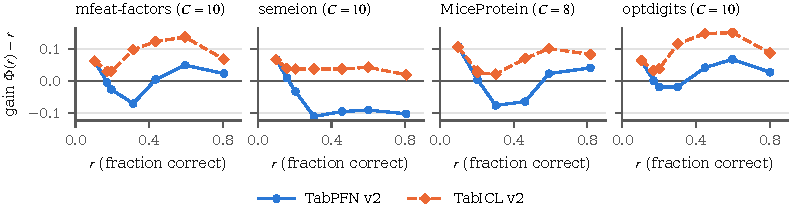
\includegraphics[width=\textwidth]{figures/mechanism_map}
\caption{Response maps for PLL at $q=0.6$ on the four Study~1 datasets with at least eight classes: gain $\Phi(r)-r$ of
one Gibbs sweep started from a fraction $r$ of correct labels, errors placed uniformly (3 seeds; needs true labels).}
\label{fig:mechanism}
\end{figure}

\subsection{Several starts and several TFMs}\label{sec:s3}
\begin{table}[t]
\centering
\caption{Study 3 (\val{s3-n-total} new datasets, four TFMs, 3 seeds). Left: registered hypotheses and criteria
(\cref{sec:design}); mean over datasets [bootstrap 95\% interval], W/T/L, one-sided Wilcoxon signed-rank $p$,
Holm-adjusted. Right: mean test score of the single chain and the multi-start average. $^\dagger$TabPFN~v2 ran only on
\val{s3-pfn2-nllp} LLP and \val{s3-pfn2-npll} PLL datasets; its row is not comparable with the others.}
\label{tab:s3}
\setlength{\tabcolsep}{3pt}
\resizebox{\textwidth}{!}{\begin{tabular}{@{}c@{\hspace{1.2em}}c@{}}% generated by paper/scripts/make_v2.py — do not edit
\begin{tabular}{@{}llll@{}}
\toprule
 & Statement & Result & Outcome \\
\midrule
H1$''$ & multi-start $>$ single chain & +0.058 [+0.016, +0.114], 13/6/1, $p$\ensuremath{<}0.001 & \textbf{confirmed} \\
H2$''$ & multi-TFM $>$ a TFM drawn at random & +0.046 [+0.019, +0.079], 18/2/0, $p$\ensuremath{<}0.001 & \textbf{confirmed} \\
H3$''$ & diagnostic AUC $\ge 0.80$ & 0.766 [0.59, 0.92] & not confirmed \\
C4$''$ & regressions $\le 10\%$ & 10/71 (14.1\%) & not met \\
C5$''$ & multi-TFM $\approx$ best TFM & gap 0.000; 1/20 worse by $>0.02$ & met \\
\bottomrule
\end{tabular}
 & % generated by paper/scripts/make_v2.py — do not edit
\begin{tabular}{@{}lrrrr@{}}
\toprule
 & \multicolumn{2}{c}{LLP, AUC (12)} & \multicolumn{2}{c}{PLL, acc.\ (8)} \\
\cmidrule(lr){2-3}\cmidrule(l){4-5}
TFM & single & multi & single & multi \\
\midrule
TabICL~v2 & 0.802 & 0.803 & 0.749 & 0.805 \\
TabPFN-3 & 0.817 & 0.817 & 0.371 & 0.650 \\
TabDPT & 0.786 & 0.799 & 0.648 & 0.720 \\
TabPFN~v2$^\dagger$ & 0.784 & 0.798 & 0.488 & 0.494 \\
\midrule
Multi-TFM & & \textbf{0.828} & & \textbf{0.808} \\
Tuned learner $L$ & \multicolumn{2}{c}{0.783} & \multicolumn{2}{c}{0.717} \\
\bottomrule
\end{tabular}
\end{tabular}}
\end{table}

\paragraph{Confirmed.} Both hypotheses of Study~3 passed (\cref{tab:s3}; per dataset in \cref{fig:s3}). Averaging three starts
improved on the single chain by \val{s3-h1-mean} on average (\val{s3-h1-wtl} datasets) \claim{14}. The gain is
concentrated: \val{s3-h1-pll} on PLL against \val{s3-h1-llp} on LLP, a median of \val{s3-h1-median} over all datasets,
and largest where single chains stall (TabPFN-3 on PLL: \val{s3-v1-tabpfn_v3-pll} to \val{s3-A1-tabpfn_v3-pll}). The
multi-TFM average improved on a TFM picked at random by \val{s3-h2-mean} (\val{s3-h2-wtl}) and was level with the best
TFM of each dataset (mean gap \val{s3-c5-gap}), more than 0.02 behind it once (\val{s3-c5-worst-name}:
\val{s3-c5-worst-X} against \val{s3-c5-worst-best}) \claim{15}. Both tests also pass without the five flagged datasets
($p_{\mathrm{Holm}}=\val{s3-s1-h1-p}$ and \val{s3-s1-h2-p}).

\paragraph{Not confirmed.} The diagnostic of H3$''$, the mean total-variation distance between the label marginals of
the warm-start and learner-start chains, reached an AUC of \val{s3-h3-auc}, below the registered 0.80. It separated
failures for TabPFN-3 (\val{s3-h3-auc-tabpfn_v3}) and TabICL~v2 (\val{s3-h3-auc-tabicl_v2}) but not for TabDPT
(\val{s3-h3-auc-tabdpt}) or TabPFN~v2 (\val{s3-h3-auc-tabpfn_v2}): we have no label-free diagnostic that transfers
across TFMs. C4$''$ also failed: with one TFM, the multi-start sampler was more than 0.02 behind the better of its
single chain and $L$ in \val{s3-c4-n} of \val{s3-n-pairs} pairs, in \val{s3-c4-vs-v1} of them behind the single chain
and in \val{s3-c4-vs-L} behind $L$ (\cref{app:s3}) \claim{18}. One TFM with several starts is thus not guaranteed to
match a tuned specialised learner; their registered descriptive comparison was not significant (\val{s3-a1L-mean},
$p=\val{s3-a1L-p}$).

\paragraph{Exploratory analysis.} The following was not registered and was computed after the confirmatory scoring
(\cref{app:s3}). (i) The multi-TFM average was above $L$ on all \val{s3x-X-L-w} datasets, by \val{s3x-X-L-mean} on
average \val{s3x-X-L-ci}, and by the measure of C4$''$ it regressed in \val{s3x-X-reg} of \val{s3-n-pairs} pairs; even
the average of single chains over TFMs, with no trained model, was above $L$ on \val{s3x-Xwarm-L-w} datasets \claim{19}.
(ii) The benefit of several starts comes from the learner start: the chain started from $L$ alone matches the
three-start average (\val{s3x-base-A1}), the cold start adds little, and averaging the single chain with $L$'s own
prediction, with no further chain, does as well as the registered average (\val{s3x-warmL-A1},
$p=\val{s3x-warmL-A1-p}$). (iii) The three chains ended within 0.03 of each other in label accuracy in
\val{s3x-basin-same} of cells; the PLL gain of the multi-start average is \val{s3x-basin-G-pll-diff} in the other cells
and \val{s3x-basin-G-pll-same} where chains agree, as \cref{thm:basins} suggests. (iv) TabICL~v2 carries much of the
multi-TFM result: the average is not significantly better than TabICL~v2's own multi-start average
(\val{s3x-X-A1-tabicl_v2}, $p=\val{s3x-X-A1-tabicl_v2-p}$); averaging over TFMs buys not having to know this in advance.

\subsection{Real weak labels, exactness and cost}\label{sec:real}\label{sec:ablation}
On three real partial-label datasets (BirdSong, Lost, MSRCv2; 10 random 90/10 splits; single chain with TabICL~v2,
registered in Study~1), \ours{} had the highest mean accuracy on all three and the best mean rank among
\val{s1-real-nmethods} methods (\val{s1-real-rank-pooled}; \cref{tab:real}) \claim{9}. The MH-corrected block sampler,
exact when the TFM is, did not predict better than the default at the same 30 sweeps (with TabICL~v2:
\val{s2e-mh-llp} AUC on LLP, \val{s2e-mh-pll6} accuracy on PLL at $q=0.6$; \cref{tab:s2e}) and was a median
\val{s2e-mh-cost-median} times slower; the comparison confounds bias with slower mixing. Chains do not mix at the level
of individual labels, and in an exploratory rerun of Study~2 with a second chain H4$'$ at $q=0.6$ no longer passes
($p_{\mathrm{Holm}}=\val{r4-b-pll6-p}$), while with the two chains averaged every test passes (\cref{tab:r4}): that
result depends on Monte Carlo variation, which averaging reduces.
On one T4 GPU a chain took a median of \val{s2-cost-median-s}\,s in Study~2 and between
\val{s3x-cost-sec-tabicl_v2}\,s (TabICL~v2) and \val{s3x-cost-sec-tabpfn_v2}\,s (TabPFN~v2) in Study~3; all chains of the
four-TFM average took a median of \val{s3x-cost-X-min} minutes per dataset and seed \claim{11}.

\section{Limitations}\label{sec:limitations}
The comparison with specialised baselines is confirmatory only for the single chain with TabICL~v2 (Study~2); the
non-neural baselines of \cref{sec:s3b} were run untuned. \Cref{thm:basins} covers the default sampler only for
instance-level weak labels with contexts that are not subsampled, and its constants are loose. Weak labels are synthetic
except for three PLL datasets, and the claims cover LLP with random bags of 8 and PLL with uniform distractors at
$q\le0.6$. Detecting a stalled chain without labels remains open.

\section{Conclusion}\label{sec:conclusion}
Under exchangeability, the predictive of an exact TFM is the full conditional of a Gibbs sampler over unknown labels,
and a real TFM approximates it. \ours{} turns this into one procedure for candidate sets and label proportions. In
Study~2 a single chain with TabICL~v2 outperformed the specialised neural and linear learners we ran on new datasets.
Averaging over starts
improved on single chains, and averaging over TFMs improved on a TFM drawn at random; in a registered supplement the
multi-TFM average also beat untuned non-neural baselines. Whether a chain stalls depends on the TFM and on where the
chain starts. Open problems: a label-free diagnostic of stalling, a cheaper way to escape a wrong start than averaging over many chains (starting
chains from a trained learner was enough in our exploratory analysis), response-map bounds with usable constants, and
feature-dependent weak labels.


\ifCLASSOPTIONcompsoc
  \section*{Acknowledgments}
\else
  \section*{Acknowledgment}
\fi
The authors used an AI assistant (Claude, Anthropic) in preparing this work, and disclose its use as IEEE policy
requires. It drafted the text of all sections and of the supplementary material from the authors' decisions and notes;
wrote the code of the method, the wrappers of the baselines and the analysis scripts that generate every number, table
and figure (\cref{sec:exp} and the supplementary material); drafted the proofs of \cref{sec:theory} and
\cref{app:proofs}, which the authors checked; and checked the references against their sources. The authors designed the
studies, approved every pre-registration and decision, ran all experiments and are responsible for all content.
\todo{confirm this disclosure; add funding, if any}


\bibliographystyle{IEEEtranN}
\bibliography{refs}

\end{document}
